\documentclass[11pt,a4paper]{article}

\usepackage{iftex}
\ifPDFTeX
  \usepackage[T1]{fontenc}
  \usepackage[utf8]{inputenc}
  \usepackage{lmodern}
\else
  \usepackage{fontspec}
\fi
\usepackage[polish]{babel}
\usepackage[a4paper,margin=2cm]{geometry}
\usepackage{graphicx}
\usepackage{float}
\usepackage{booktabs}
\usepackage{array}
\usepackage{amsmath}
\usepackage{tabularx}
\usepackage{xcolor}
\usepackage[font=small,labelfont=bf]{caption}
\usepackage{enumitem}
\usepackage{microtype}
\usepackage{fancyhdr}
\usepackage[hidelinks]{hyperref}

\graphicspath{{img/}}
\setlist{itemsep=2pt,topsep=4pt}
\setlength{\parskip}{4pt}
\setlength{\parindent}{0pt}
\setlength{\emergencystretch}{3em}

\pagestyle{fancy}
\fancyhf{}
\lhead{\small Projekt -- System moderacji komentarzy z wykorzystaniem LLM}
\rhead{\small Dawid Olko}
\cfoot{\thepage}
\setlength{\headheight}{14pt}

\newcommand{\zrzut}[2]{%
  \begin{figure}[H]
    \centering
    \setlength{\fboxsep}{2pt}%
    \fcolorbox{black!25}{white}{\includegraphics[width=\dimexpr\linewidth-6pt\relax,height=0.8\textheight,keepaspectratio]{#1}}
    \caption{#2}
    \label{fig:#1}
  \end{figure}}

\newcommand{\kod}[1]{\texttt{\hyphenchar\font=`\-\relax #1}}


\begin{document}
\begin{titlepage}
  \centering
  \vspace*{3cm}
  {\large Uniwersytet Rzeszowski\par}
  \vspace{0.2cm}
  {\large Wydział Nauk Ścisłych i Technicznych\par}
  \vspace{0.5cm}
  {\large Wprowadzenie do dużych modeli językowych\par}
  \vspace{2.5cm}
  {\LARGE\bfseries Projekt zaliczeniowy\par}
  \vspace{0.6cm}
  {\Large System moderacji komentarzy z wykorzystaniem LLM\par}
  \vspace{3cm}
  {\large Dawid Olko\par}
  \vspace{0.2cm}
  {\large Nr albumu: 125148\par}
  \vfill
  {\large Rzeszów, 23 listopada 2026\par}
\end{titlepage}


\tableofcontents
\newpage

\section{Cel projektu}

Celem projektu była aplikacja w Pythonie, która pomaga moderatorowi forum internetowego. Aplikacja ocenia komentarze
(obraźliwe, wulgarne, groźby, mowa nienawiści, spam), uzasadnia decyzję cytatem z regulaminu forum, czyta komentarze
w postaci obrazków (memy, zrzuty ekranu), przetwarza całe pliki komentarzy i pozwala rozmawiać z modelem o wczytanym
pliku. Wszystkie modele działają lokalnie w Ollamie, bez płatnych usług i bez karty graficznej. Temat jest rozwinięciem
tematu 15 z listy (,,Detektor toksyczności komentarzy online'') i łączy się z laboratorium 2, gdzie używałem modelu
\kod{unitary/toxic-bert}.

Projekt ma dwa interfejsy, które korzystają z tego samego kodu: polecenie \kod{moderator} w terminalu oraz aplikację
webową w Gradio. Całość uruchamia się jednym poleceniem w Dockerze.

Wymagania prowadzącego zrealizowałem po kolei, od oceny 3.0 do 5.0, w jednym projekcie:

\begin{table}[H]
\centering
\small
\begin{tabularx}{\linewidth}{@{}l X l@{}}
\toprule
Ocena & Wymaganie i realizacja & Rozdział \\
\midrule
3.0 & Ollama jako gotowe narzędzie, kroki konfiguracji, znaczenie parametrów z eksperymentem, klasyfikacja
      pojedynczego komentarza promptem (\kod{moderator classify}) & \ref{sec:srodowisko}, \ref{sec:parametry}, \ref{sec:klasyfikacja} \\
3.5 & Wielomodalność: model \kod{gemma3:4b} czyta tekst z obrazka, a potem komentarz jest oceniany jak tekst
      (\kod{moderator image}) & \ref{sec:obrazy} \\
4.0 & Automatyzacja: hurtowa moderacja pliku CSV lub TXT do pliku CSV z oceną i uzasadnieniem
      (\kod{moderator batch}) & \ref{sec:wsadowo} \\
4.5 & Rozmowa przez API Ollamy o przesłanym pliku \kod{.txt} z historią, promptem systemowym i few-shot; zapis
      raportu \kod{.txt} i wykresu \kod{.svg} (\kod{moderator chat}) & \ref{sec:czat} \\
5.0 & RAG: wyszukiwanie paragrafów regulaminu (BM25, embeddingi, ranking hybrydowy) i decyzja z cytatem
      \kod{§}; porównanie z wersją bez RAG (\kod{moderator rag}, \kod{moderator evaluate}) & \ref{sec:rag}, \ref{sec:ewaluacja} \\
\bottomrule
\end{tabularx}
\caption{Wymagania na oceny i miejsce ich realizacji.}
\end{table}

Kod jest w repozytorium \url{https://github.com/dawidolko/CommentModerator-LLM-Python}. Wszystkie liczby
i przykłady w tym sprawozdaniu pochodzą z prawdziwych uruchomień, a ich pliki wynikowe są w katalogu
\kod{examples/}.

\section{Krótko o teorii}

\textbf{Moderacja treści} to decyzja, czy wpis może zostać na forum. W praktyce nie wystarczy etykieta
,,toksyczny / nietoksyczny'' -- moderator musi wiedzieć, \emph{co} jest nie tak i \emph{na jakiej podstawie} usuwa
wpis. Dlatego każda odpowiedź modelu ma w projekcie stały format: kategorie, stopień naruszenia (0--3), decyzję
(\kod{allow}, \kod{review}, \kod{remove}), krótkie uzasadnienie i -- w trybie RAG -- numer paragrafu regulaminu.

\textbf{Model instrukcyjny} (tutaj Qwen 2.5 7B) był po pretreningu dostrojony do wykonywania poleceń. W odróżnieniu od
GPT-2 z laboratorium 1 nie ,,dopisuje'' dalszego ciągu tekstu, tylko odpowiada na polecenie, więc można go poprosić
o ocenę komentarza w ustalonym formacie.

\textbf{Inżynieria promptów} to dobór treści wysyłanej do modelu. W projekcie używam:
\begin{itemize}
  \item \textbf{promptu systemowego} z rolą (,,moderator polskiego forum programistów''), definicjami kategorii
        i zasadą wyboru decyzji,
  \item \textbf{few-shot}, czyli kilku przykładowych par komentarz -- odpowiedź JSON, po polsku i po angielsku,
  \item \textbf{wymuszonego formatu}: Ollama przyjmuje schemat JSON (\kod{format}) i ogranicza generowanie tak,
        żeby odpowiedź była zgodna ze schematem,
  \item \textbf{niskiej temperatury i stałego ziarna} -- wniosek z laboratorium 5: przy $T=0{,}3$ odpowiedzi były
        znacznie wierniejsze niż przy $T=1{,}0$.
\end{itemize}

\textbf{RAG} (\emph{Retrieval-Augmented Generation}) polega na tym, że przed odpowiedzią wyszukuje się fragmenty
dokumentów pasujące do pytania i wkleja je do promptu. Model odpowiada wtedy na podstawie tych fragmentów, a nie tylko
własnej wiedzy. Tutaj dokumentem jest regulamin forum, a fragmentem -- pojedynczy paragraf (\kod{§2.1}, \kod{§5.2}
itd.). Do wyszukiwania używam trzech metod:
\begin{itemize}
  \item \textbf{BM25} -- klasyczny ranking leksykalny z laboratorium 3; liczy wspólne słowa zapytania i dokumentu
        z poprawką na częstość słowa i długość dokumentu,
  \item \textbf{embeddingi} (\kod{nomic-embed-text}) -- tekst zamieniany jest na wektor, a podobieństwo liczy się
        jako cosinus kąta między wektorami; działa także przy innych słowach o podobnym znaczeniu,
  \item \textbf{ranking hybrydowy RRF} (\emph{Reciprocal Rank Fusion}) -- łączy oba rankingi wzorem
        $\sum 1/(k + \text{pozycja})$ z $k = 60$.
\end{itemize}

\textbf{Model bazowy} \kod{unitary/toxic-bert} to BERT dostrojony na komentarzach z Wikipedii do 6 etykiet
(klasyfikacja wieloetykietowa, więc sigmoid i osobny próg dla etykiety, tak jak w laboratorium 2.3). Służy do
porównania: jest szybki, ale zna tylko angielski i nie umie uzasadnić decyzji.

\section{Architektura}
\label{sec:architektura}

Kod jest pakietem Pythona \kod{moderator} w katalogu \kod{src/}. Każdy plik robi jedną rzecz, a terminal i aplikacja
webowa korzystają z jednej klasy \kod{Moderator} (plik \kod{service.py}), więc wynik jest taki sam niezależnie od
interfejsu.

\begin{table}[H]
\centering
\small
\begin{tabularx}{\linewidth}{@{}l X@{}}
\toprule
Plik & Zadanie \\
\midrule
\kod{config.py} & wczytanie \kod{config.yaml} i zmiennych środowiskowych (\kod{.env}) \\
\kod{llm.py} & klient Ollamy: czat, czat strumieniowy, obraz, embeddingi \\
\kod{schema.py} & schemat odpowiedzi (Pydantic) i jego walidacja \\
\kod{prompts.py} & prompt systemowy, przykłady few-shot, szablony RAG, odczytu obrazu i czatu \\
\kod{classify.py} & ocena komentarza (zero-shot, few-shot) z ponowieniem przy złym JSON-ie \\
\kod{rules.py}, \kod{retrieval.py}, \kod{rag.py} & podział regulaminu na paragrafy, BM25, embeddingi, RRF, ocena z cytatem \\
\kod{vision.py} & odczyt tekstu z obrazka modelem wizyjnym \\
\kod{baseline.py} & model bazowy \kod{unitary/toxic-bert} \\
\kod{batch.py}, \kod{report.py} & moderacja pliku, raport \kod{.txt}, wykres \kod{.svg} \\
\kod{chat.py} & sesja rozmowy o pliku z historią i komendami \\
\kod{evaluate.py} & metryki porównania wariantów \\
\kod{cli/} & polecenia terminala (Typer + Rich), podzielone na \kod{single}, \kod{files}, \kod{tools}, \kod{views} \\
\kod{web/} & aplikacja Gradio; każda zakładka w osobnym pliku w \kod{web/tabs/} \\
\bottomrule
\end{tabularx}
\caption{Moduły pakietu \kod{moderator}.}
\end{table}

Przepływ jednego komentarza w trybie RAG wygląda tak:
\begin{enumerate}
  \item (tylko obrazek) \kod{gemma3:4b} odczytuje tekst z obrazka,
  \item wyszukiwarka zwraca 3 najlepsze paragrafy regulaminu; do kontekstu zawsze dochodzi też \kod{§2.3}
        (dozwolona krytyka), żeby model miał podstawę do zostawienia wpisu,
  \item \kod{qwen2.5:7b} dostaje prompt systemowy, przykłady few-shot, paragrafy i komentarz, a odpowiada JSON-em
        zgodnym ze schematem,
  \item odpowiedź jest sprawdzana: zły JSON -- jedna ponowna próba, potem decyzja \kod{review}; paragraf, którego
        nie ma w regulaminie, albo usunięcie bez paragrafu -- decyzja zmieniana na \kod{review}.
\end{enumerate}

Dane są w całości syntetyczne: 40 komentarzy (23 po polsku, 17 po angielsku, 22 naruszające zasady) w
\kod{data/comments.csv} z etykietą, kategorią i właściwym paragrafem, fikcyjny regulamin forum ,,Kod po godzinach''
(14 paragrafów w \kod{data/rules/forum\_rules.md}) oraz 6 obrazków wygenerowanych skryptem
\kod{scripts/make\_sample\_images.py}. Komentarze toksyczne są celowo łagodne i nie zawierają prawdziwych wyzwisk wobec
grup.

\section{Konfiguracja środowiska}
\label{sec:srodowisko}

Projekt uruchamiałem na MacBooku Pro M3 Pro z 18 GB pamięci. Ollama 0.32.6 działa natywnie (Metal), aplikacja
w Pythonie 3.12. Dokładne wersje bibliotek są przypięte w \kod{requirements.txt}.

\subsection{Docker}

Najprostsza droga to Docker Compose. Plik \kod{.tools/docker/docker-compose.yml} ma trzy usługi:
\begin{itemize}
  \item \kod{ollama} -- oficjalny obraz \kod{ollama/ollama:0.32.6}, modele trzymane w wolumenie \kod{ollama},
  \item \kod{models} -- uruchamia się raz, pobiera trzy modele (\kod{ollama pull}) i kończy działanie,
  \item \kod{app} -- obraz z aplikacją (Python 3.12, PyTorch w wersji CPU), startuje po pobraniu modeli i wystawia
        aplikację webową na porcie 7860.
\end{itemize}

\begin{verbatim}
docker compose -f .tools/docker/docker-compose.yml up --build
docker compose -f .tools/docker/docker-compose.yml exec app moderator check
\end{verbatim}

Na macOS Docker nie ma dostępu do GPU, więc Ollama w kontenerze liczy na procesorze. Sprawdziłem cały stos w tej
konfiguracji: ta sama groźba w trybie RAG dostała w kontenerze ten sam werdykt (\kod{remove}, §3.1), ale ocena trwała
37,8~s zamiast 4,8~s przy Ollamie uruchomionej natywnie.
Dlatego na Macu kontener aplikacji może korzystać z Ollamy zainstalowanej natywnie (zmienna \kod{OLLAMA\_HOST}
wskazuje na \kod{host.docker.internal}). Skrypt \kod{start.sh} wybiera ten wariant sam, gdy wykryje działającą Ollamę.

\subsection{Python bez Dockera}

\begin{verbatim}
python3 -m venv .venv
source .venv/bin/activate
pip install -r requirements.txt
pip install -e .
ollama pull qwen2.5:7b
ollama pull gemma3:4b
ollama pull nomic-embed-text
moderator check
\end{verbatim}

Polecenie \kod{pip install -e .} instaluje pakiet i komendę \kod{moderator}. Ustawienia są w dwóch plikach:
\kod{config.yaml} (modele, parametry generowania, wyszukiwanie, ścieżki) i \kod{.env} (adres Ollamy i nazwy modeli,
wzór w \kod{.env.example}). Zmienna \kod{HF\_HUB\_DISABLE\_XET=1} omija błędy pobierania z Hugging Face, na które
trafiłem na laboratoriach.

\zrzut{code_settings}{Kod: wczytanie ustawień z \kod{config.yaml} i zmiennych środowiskowych.}

Polecenie \kod{moderator check} sprawdza połączenie z Ollamą i to, czy modele są pobrane:

\zrzut{check}{Wynik: \kod{moderator check}.}

\subsection{Modele}

\begin{table}[H]
\centering
\small
\begin{tabular}{@{}llll@{}}
\toprule
Rola & Model & Rozmiar & Dlaczego \\
\midrule
tekst & \kod{qwen2.5:7b} & 4,7 GB & dobrze radzi sobie z polskim, trzyma się schematu JSON \\
obraz & \kod{gemma3:4b} & 3,3 GB & czyta tekst z obrazków, mieści się w 18 GB razem z modelem tekstowym \\
embeddingi & \kod{nomic-embed-text} & 0,3 GB & wektory do wyszukiwania paragrafów regulaminu \\
model bazowy & \kod{unitary/toxic-bert} & 0,4 GB & porównanie z laboratorium 2 \\
\bottomrule
\end{tabular}
\caption{Modele użyte w projekcie.}
\end{table}

Klient Ollamy jest w pliku \kod{llm.py}. Ma cztery metody: zwykły czat (opcjonalnie ze schematem JSON), czat
strumieniowy do rozmowy, zapytanie z obrazkiem i embeddingi. Parametr \kod{keep\_alive="30m"} trzyma model w pamięci
między zapytaniami, więc przy przetwarzaniu pliku model nie ładuje się od nowa.

\zrzut{code_llm}{Kod: klient Ollamy (\kod{llm.py}).}

\newpage
\section{Parametry Ollamy}
\label{sec:parametry}

Każde zapytanie do Ollamy ma obiekt \kod{options}. Wartości używane w aplikacji są w \kod{config.yaml}: sekcja
\kod{generation} dla moderacji (krótkie, powtarzalne odpowiedzi JSON) i sekcja \kod{chat} dla rozmowy (dłuższy,
trochę swobodniejszy tekst).

\begin{table}[H]
\centering
\small
\begin{tabularx}{\linewidth}{@{}l l X@{}}
\toprule
Parametr & Wartość & Znaczenie \\
\midrule
\kod{temperature} & 0,1 (czat 0,3) & dzieli logity przed losowaniem; mała wartość -- prawie zawsze wygrywa najbardziej
  prawdopodobny token, duża -- rozkład się spłaszcza i tekst jest bardziej różnorodny \\
\kod{top\_p} & 0,9 & \emph{nucleus sampling}: losowanie tylko z najmniejszego zbioru tokenów, których
  prawdopodobieństwa sumują się do \kod{top\_p} \\
\kod{top\_k} & 40 & losowanie tylko z \kod{top\_k} najbardziej prawdopodobnych tokenów; \kod{top\_k = 1} to
  dekodowanie zachłanne (\emph{greedy}) z laboratorium 1 \\
\kod{seed} & 42 & stałe ziarno generatora losowego -- ten sam prompt i te same opcje dają tę samą odpowiedź \\
\kod{num\_ctx} & 4096 (czat 8192) & okno kontekstu w tokenach; muszą się w nim zmieścić prompt, przykłady,
  paragrafy i odpowiedź \\
\kod{num\_predict} & 300 (czat 700) & maksymalna liczba wygenerowanych tokenów \\
\kod{repeat\_penalty} & 1,1 & obniża prawdopodobieństwo tokenów, które już wystąpiły (przeciw pętlom, które
  robił GPT-2) \\
\kod{stop} & brak & napisy, na których generowanie się kończy \\
\kod{format} & schemat JSON & ogranicza generowanie do poprawnego JSON-a zgodnego ze schematem \\
\kod{keep\_alive} & 30 min & jak długo model zostaje w pamięci po ostatnim zapytaniu \\
\bottomrule
\end{tabularx}
\caption{Parametry generowania w Ollamie.}
\end{table}

\subsection{Eksperyment}

Skrypt \kod{scripts/parameter\_experiment.py} wysyła do \kod{qwen2.5:7b} te same zapytania z różnymi opcjami i zapisuje
wyniki w \kod{examples/parameters/parameters.json}. Ziarno jest w nim domyślnie wyłączone, żeby było widać naturalną
zmienność modelu. Wyniki jednego uruchomienia:

\begin{table}[H]
\centering
\small
\begin{tabularx}{\linewidth}{@{}>{\raggedright\arraybackslash}p{0.4\linewidth} X@{}}
\toprule
Test & Wynik \\
\midrule
\kod{temperature} 0 / 0,7 / 1,5, ocena komentarza ,,Kurde, znowu zapomniałem średnika'' 5 razy (schemat JSON)
  & za każdym razem \kod{review}, stopień 1 -- przy wymuszonym schemacie i jasnym prompcie decyzja nie zmieniła się
    nawet przy $T = 1{,}5$ \\
\kod{seed} przy $T = 0{,}9$, 3 odpowiedzi tekstowe & z ziarnem 42: 1 różna odpowiedź na 3, bez ziarna: 3 różne na 3 \\
\kod{top\_p} 0,1 / 1,0 przy $T = 1{,}0$, 5 odpowiedzi & 1 / 5 różnych odpowiedzi \\
\kod{top\_k} 1 / 100 przy $T = 1{,}0$, 5 odpowiedzi & 1 / 5 różnych odpowiedzi \\
\kod{num\_predict = 15} & odpowiedź urwana w połowie: \kod{\{ "toxic": false, "categories": ["none"], "severity} --
  takiego JSON-a nie da się odczytać \\
\kod{format}: brak / \kod{"json"} / schemat, 5 komentarzy & poprawne oceny: 0 / 0 / 5 na 5; bez schematu model
  zwracał skrócony JSON, np. \kod{\{"toxic": true, "reason": "insult"\}} \\
\kod{num\_ctx} 2048 / 16384, krótki prompt & 1,26 s / 1,26 s -- przy krótkim prompcie rozmiar okna nie wpływa na czas,
  ma znaczenie dopiero przy długim wejściu (czat o pliku) i dla zajętości pamięci \\
\kod{stop = [","]} & odpowiedź kończy się przed pierwszym przecinkiem \\
\bottomrule
\end{tabularx}
\caption{Wpływ parametrów -- wyniki \kod{scripts/parameter\_experiment.py}.}
\end{table}

Najważniejszy wniosek jest taki, że o powtarzalności decyzji bardziej decyduje wymuszony schemat (\kod{format}) niż
sama temperatura. Temperatura, \kod{top\_p} i \kod{top\_k} wyraźnie zmieniają za to swobodny tekst -- dlatego w czacie
temperatura jest trochę wyższa niż przy moderacji, a ziarno jest stałe w obu przypadkach.

\newpage
\section{Ocena pojedynczego komentarza (3.0)}
\label{sec:klasyfikacja}

\subsection{Format odpowiedzi}

Każda ocena ma ten sam kształt, opisany klasą \kod{Verdict} w \kod{schema.py}. Z tej samej klasy powstaje schemat
JSON przekazywany do Ollamy w parametrze \kod{format}, więc model nie może zwrócić kategorii spoza listy ani stopnia
spoza zakresu 0--3. Walidator porządkuje drobiazgi: usuwa powtórzone kategorie, usuwa \kod{none} obok prawdziwej
kategorii i dopisuje znak \kod{§} do numeru paragrafu.

\zrzut{code_schema}{Kod: schemat odpowiedzi (\kod{schema.py}).}

\subsection{Prompt}

Prompt składa się z trzech części. Prompt systemowy ustawia rolę moderatora, definiuje sześć kategorii, stopnie
naruszenia i zasadę wyboru decyzji, a także mówi wprost, że rzeczowa krytyka i potoczne zwroty (,,I could kill for
a coffee'') nie są naruszeniem. Potem idzie pięć przykładów few-shot -- dwa po angielsku, trzy po polsku, w tym dwa
dozwolone (rzeczowa uwaga i frustracja), żeby model nie uznawał każdego ostrego słowa za obelgę. Na końcu jest
komentarz w potrójnym cudzysłowie, żeby model nie pomylił treści komentarza z poleceniem.

\zrzut{code_prompt}{Kod: składanie wiadomości dla modelu (\kod{prompts.py}).}

Tryb \kod{zero-shot} wysyła tylko prompt systemowy i komentarz, tryb \kod{few-shot} dokłada przykłady. Jeśli
odpowiedzi nie da się odczytać jako JSON zgodny ze schematem, zapytanie jest ponawiane raz, a potem wynik dostaje
decyzję \kod{review} z notatką o błędzie. Komentarz trafia wtedy do człowieka, zamiast zostać po cichu przepuszczony.

\zrzut{code_classify}{Kod: zapytanie o ocenę z ponowieniem (\kod{classify.py}).}

\subsection{Przykłady}

Komentarz z obelgą w trybie zero-shot:

\zrzut{classify_insult}{Wynik: \kod{moderator classify} w trybie zero-shot.}

Komentarz z idiomem ,,I could kill for a coffee'' w trybie few-shot (domyślnym). Model rozpoznał, że to nie groźba:

\zrzut{classify_idiom}{Wynik: \kod{moderator classify} dla idiomu.}

Dla porównania ten sam komentarz w modelu bazowym \kod{unitary/toxic-bert} z laboratorium 2:

\zrzut{bert_idiom}{Wynik: \kod{moderator bert} dla idiomu.}

Tutaj oba modele zgadzają się, że idiom nie jest groźbą (najwyższy wynik toxic-bert to 0,009). Różnica jest
w tym, że toxic-bert zwraca tylko liczby dla sześciu etykiet, a model językowy także decyzję i uzasadnienie. Widać też
słabość małego modelu: uzasadnienia po polsku zdarzają się z błędami językowymi (,,Idioma wyrażające\ldots'',
,,Niezaskomlone oskarżenie\ldots''), mimo że sama decyzja jest trafna.

\newpage
\section{Komentarze w postaci obrazków (3.5)}
\label{sec:obrazy}

Na forach część treści to memy i zrzuty ekranu, których zwykły klasyfikator tekstu nie przeczyta. Dlatego ocena
obrazka ma dwa kroki. Najpierw model wizyjny \kod{gemma3:4b} dostaje obrazek i polecenie: ,,przepisz cały tekst
z obrazka i jednym zdaniem opisz, co przedstawia''. Odpowiedź ma ustalony układ (\kod{TEXT:} i \kod{PICTURE:}), z którego
wycinam tekst. Potem ten tekst przechodzi przez tę samą ocenę co zwykły komentarz (domyślnie w trybie RAG).

Mały model wizyjny czasem powtarzał tę samą linię dwa razy albo dopisywał etykietę \kod{TEXT:} w środku odpowiedzi.
Funkcja \kod{clean\_text} usuwa etykiety i powtórzone linie, a następnie skleja tekst w jedno zdanie.

\zrzut{code_vision}{Kod: odczyt tekstu z obrazka i ocena (\kod{vision.py}).}

Obrazki testowe wygenerowałem skryptem \kod{scripts/make\_sample\_images.py} (Pillow): trzy memy z tekstem na górze
i na dole oraz trzy zrzuty ekranu wpisu z forum. Dzięki temu nie używam cudzych materiałów.

\begin{figure}[H]
  \centering
  
\includegraphics[width=0.45\linewidth]{meme_03.png}\hfill
  
\includegraphics[width=0.52\linewidth]{screenshot_01.png}
  \caption{Przykładowe obrazki: mem z groźbą i zrzut ekranu ze spamem.}
\end{figure}

\zrzut{image_meme}{Wynik: \kod{moderator image data/images/meme\_03.png}.}

\zrzut{image_screenshot}{Wynik: \kod{moderator image data/images/screenshot\_01.png}.}

Model wizyjny przeczytał oba obrazki poprawnie, z jednym błędem: na memie ,,NAPISZ'' odczytał jako ,,NAPIS''.
Dla oceny nie miało to znaczenia -- komentarz dostał kategorię \kod{threat}, stopień 3 i paragraf §3.1, a reklama ze
zrzutu ekranu kategorię \kod{spam} i paragraf §5.1. Ocena obrazka trwa około 16--18 sekund, bo do pamięci trzeba
załadować dwa modele.

\section{Moderacja całego pliku (4.0)}
\label{sec:wsadowo}

Polecenie \kod{moderator batch} wczytuje plik CSV z kolumną \kod{text} (albo plik TXT, jeden komentarz w linii),
ocenia komentarze po kolei z paskiem postępu i zapisuje CSV z kolumnami \kod{id, text, toxic, categories, severity,
decision, reason, rule, latency\_s}. Obok zapisuje raport \kod{report.txt} i wykres \kod{chart.svg}.

\zrzut{code_batch}{Kod: moderacja tabeli komentarzy (\kod{batch.py}).}

\zrzut{batch}{Wynik: \kod{moderator batch data/comments.csv -o examples/batch/moderated.csv}.}

Cały plik 40 komentarzy (tryb few-shot) zajął około 80 sekund, średnio 2,0 s na komentarz. Wynik: 17 komentarzy
zostawionych, 3 do sprawdzenia, 20 do usunięcia. Pliki tego uruchomienia są w \kod{examples/batch/}
(\kod{moderated.csv}, \kod{report.txt}, \kod{chart.svg}).

\newpage
\section{Rozmowa o pliku z komentarzami (4.5)}
\label{sec:czat}

Polecenie \kod{moderator chat data/comments.txt} (oraz zakładka \emph{Chat about a file} w aplikacji) pozwala zadawać
modelowi pytania o wczytany plik. Cały plik nie trafia do modelu jako surowy tekst. Najpierw każdy komentarz jest
oceniany (w trybie RAG), a wynik zapisuje się w pamięci podręcznej \kod{out/cache/}, więc drugie wczytanie tego
samego pliku jest natychmiastowe. Potem prompt systemowy dostaje tabelę z numerem, decyzją, kategoriami, stopniem,
paragrafem, uzasadnieniem i treścią każdego komentarza. Model odpowiada na podstawie tej tabeli i podaje numery
komentarzy (\kod{\#9}).

Inżynieria promptów w czacie:
\begin{itemize}
  \item prompt systemowy z rolą (,,pomagasz moderatorowi przejrzeć plik''), zasadą odpowiadania w języku pytania,
        cytowania numerów i przyznawania się, gdy tabela nie zawiera odpowiedzi,
  \item historia rozmowy -- każde pytanie i odpowiedź są dopisywane do listy wiadomości, więc można dopytać
        (,,a który z nich jest najgorszy?''),
  \item odpowiedź przychodzi strumieniowo (\kod{stream=True}), parametry z sekcji \kod{chat} w \kod{config.yaml}
        (temperatura 0,3, okno kontekstu 8192 tokeny).
\end{itemize}

Komendy w czacie: \kod{/report} zapisuje raport \kod{report.txt}, \kod{/chart} zapisuje wykres \kod{chart.svg},
\kod{/save} zapisuje rozmowę, \kod{/exit} kończy rozmowę (i też ją zapisuje).

\zrzut{code_chat}{Kod: sesja rozmowy o pliku (\kod{chat.py}).}

\subsection{Przykładowa rozmowa}

Skrypt \kod{scripts/chat\_example.py} zadaje cztery pytania o plik \kod{data/comments.txt}; pełny zapis jest
w \kod{examples/chat/chat\_log.txt}, a raport i wykres w tym samym katalogu.

\begin{itemize}
  \item ,,Które komentarze są groźbami i dlaczego?'' -- model wymienił \#9, \#10 i \#35 z uzasadnieniem.
        Pominął \#22 (,,Someone should beat up the guy\ldots''), który przy moderacji też dostał kategorię
        \kod{threat}.
  \item ,,A który z nich jest najpoważniejszy?'' -- pytanie odwołuje się do poprzedniej odpowiedzi i model to
        zrozumiał dzięki historii; wskazał \#10 ze stopniem 3 (ten sam stopień ma też \#35, czego nie wspomniał).
  \item ,,Which comments look like spam\ldots?'' -- odpowiedź po angielsku, cztery komentarze z paragrafami.
  \item ,,Ile komentarzy trzeba usunąć\ldots?'' -- tu model się pomylił: wypisał 17 komentarzy i źle policzył
        kategorie, a według raportu do usunięcia jest 22.
\end{itemize}

To typowe zachowanie modelu językowego: dobrze znajduje i tłumaczy konkretne wpisy, ale słabo liczy po długiej
tabeli. Dlatego liczby w raporcie \kod{/report} liczy kod, a nie model.

\begin{figure}[H]
  \centering
  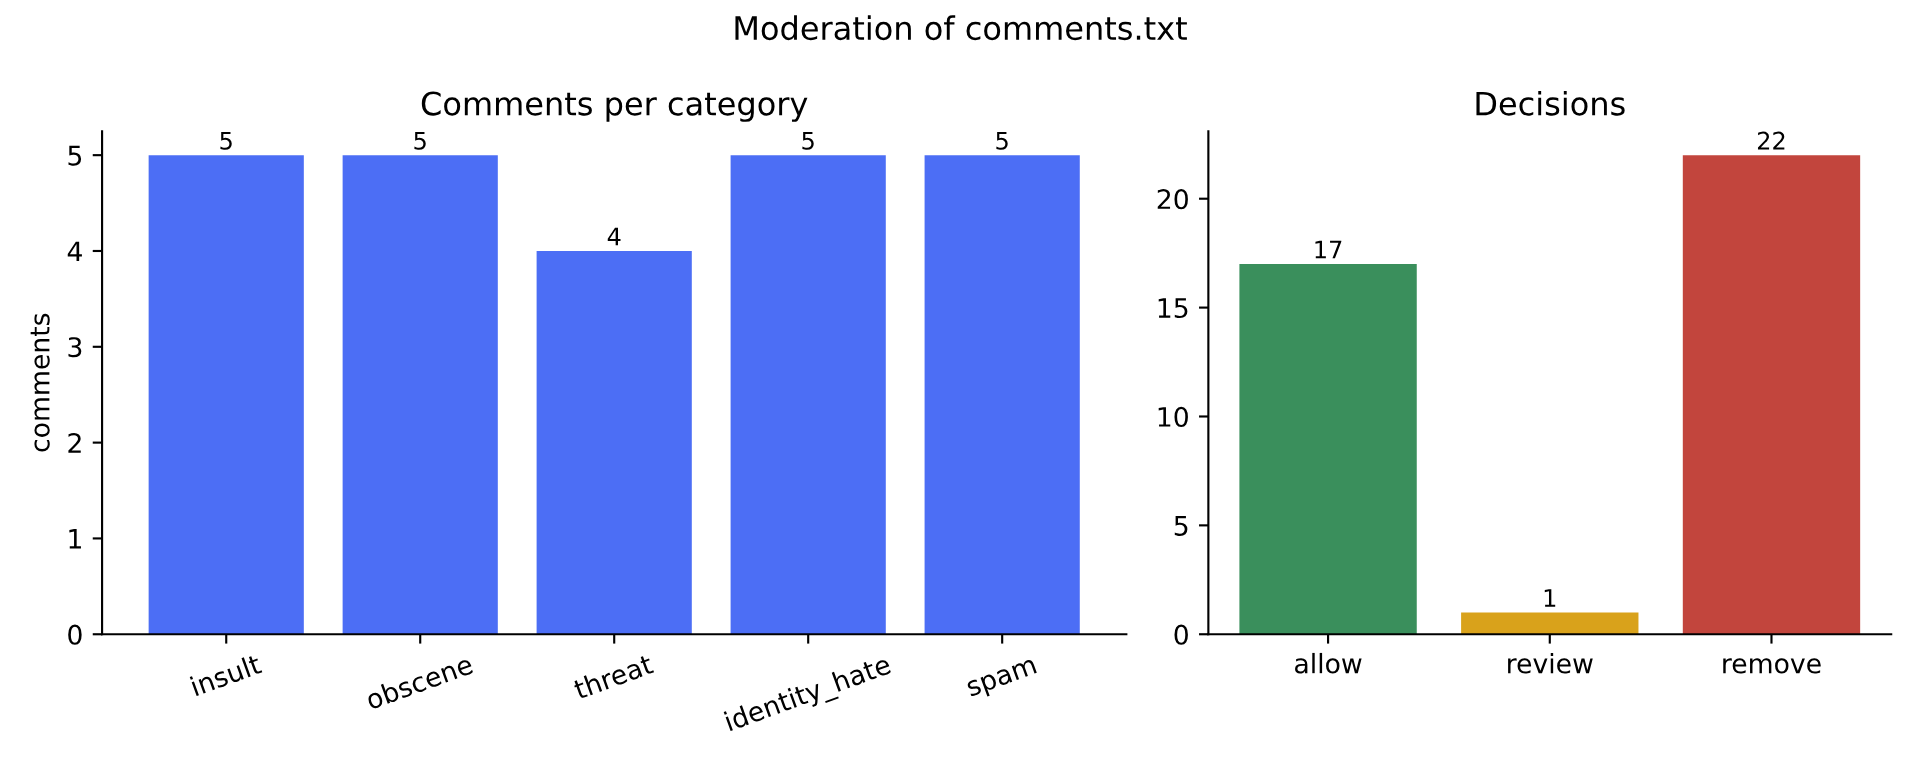
\includegraphics[width=\linewidth]{chart.png}
  \caption{Wykres zapisany komendą \kod{/chart} (\kod{examples/chat/chart.svg}).}
\end{figure}

\newpage
\section{RAG na regulaminie forum (5.0)}
\label{sec:rag}

Moderator, który usuwa wpis, powinien wskazać złamany punkt regulaminu. Model sam z siebie nie zna regulaminu tego
konkretnego forum, więc w trybie RAG dostaje jego fragmenty w prompcie.

\subsection{Baza wiedzy}

Regulamin \kod{data/rules/forum\_rules.md} ma 6 rozdziałów i 14 paragrafów. Plik \kod{rules.py} dzieli go na paragrafy
po nagłówkach \kod{\#\#\# §X.Y}; każdy paragraf to jeden dokument. Rozdziały §1 (postanowienia ogólne) i §6 (zasady
moderacji) nie opisują zachowań użytkowników, więc nie biorą udziału w wyszukiwaniu (\kod{skip\_sections} w
\kod{config.yaml}). Regulamin jest po polsku, ale część komentarzy jest po angielsku, dlatego na końcu paragrafów
dopisałem w nawiasie krótki angielski opis.

\subsection{Wyszukiwanie}

\kod{retrieval.py} ma trzy metody. BM25 działa na słowach po prostym ujednoliceniu: małe litery, usunięte polskie znaki
i obcięcie słowa do 5 pierwszych liter (prymitywny stemming, który łączy np. ,,groźby'' i ,,grożenie''). Wyszukiwanie
wektorowe używa \kod{nomic-embed-text} z prefiksami \kod{search\_document:} i \kod{search\_query:}, których ten model
wymaga. Metoda hybrydowa łączy oba rankingi przez RRF.

\zrzut{code_retrieval}{Kod: wyszukiwarka paragrafów (\kod{retrieval.py}).}

\subsection{Ocena z cytatem}

Do promptu trafiają 3 najlepsze paragrafy oraz zawsze §2.3 (dozwolona krytyka), żeby przy zwykłym komentarzu model
miał paragraf, na który może się powołać. W schemacie JSON pole \kod{rule} ma listę dozwolonych wartości
(\kod{enum}) równą numerom znalezionych paragrafów, więc model nie może wymyślić paragrafu. Na koniec kod sprawdza
odpowiedź jeszcze raz: paragraf spoza regulaminu albo usunięcie bez paragrafu zmienia decyzję na \kod{review}.

\zrzut{code_rag}{Kod: ocena komentarza z regulaminem (\kod{rag.py}).}

Pierwsza wersja nie miała listy \kod{enum}, a w instrukcji było ,,podaj paragraf albo null''. Model bardzo często
wybierał \kod{null}, także przy oczywistej groźbie, i takie komentarze trafiały do \kod{review} zamiast do
\kod{remove}. Ograniczenie pola w schemacie rozwiązało ten problem -- wyniki obu wersji są w rozdziale
\ref{sec:ewaluacja}.

\subsection{Przykłady}

\zrzut{rag_spam}{Wynik: \kod{moderator rag} dla reklamy z kodem rabatowym.}

\zrzut{rag_threat}{Wynik: \kod{moderator rag} dla groźby.}

\newpage
\section{Ewaluacja}
\label{sec:ewaluacja}

Polecenie \kod{moderator evaluate} porównuje na 40 oznaczonych komentarzach pięć wariantów:
\begin{itemize}
  \item \kod{unitary/toxic-bert} z progiem 0,5 i z progiem z krzywej precision--recall (punkt, w którym precision
        $\approx$ recall -- tak jak w laboratorium 2.3),
  \item LLM zero-shot, few-shot i RAG.
\end{itemize}
Metryki: precision, recall i F1 dla klasy ,,naruszenie'', zgodność kategorii (czy właściwa kategoria jest wśród
przewidzianych), zgodność paragrafu (tylko RAG) i średni czas na komentarz. Osobno mierzę, czy wyszukiwarka znajduje
właściwy paragraf (Recall@1, Recall@3, MRR). Wyniki są w \kod{examples/evaluation/}.

\subsection{Pierwsze uruchomienie}

Pierwsze uruchomienie pokazało dwa błędy w moim prompcie i schemacie:

\begin{table}[H]
\centering
\small
\begin{tabular}{@{}lccccc@{}}
\toprule
Wariant & Precision & Recall & F1 & Kategoria & Paragraf \\
\midrule
LLM zero-shot & 0,947 & 0,818 & 0,878 & 0,925 & -- \\
LLM few-shot & 0,957 & 1,000 & 0,978 & 0,950 & -- \\
LLM RAG & 0,957 & 1,000 & 0,978 & 0,925 & 0,600 \\
\bottomrule
\end{tabular}
\caption{Pierwsze uruchomienie (\kod{examples/evaluation\_first\_run.md}).}
\end{table}

\begin{itemize}
  \item W trybie zero-shot cztery komentarze ze spamem dostały \kod{toxic: false}, chociaż decyzja brzmiała
        \kod{remove}. Bez definicji model rozumiał ,,toxic'' jako ,,niegrzeczny'', a spam nie jest niegrzeczny.
        Dopisałem do promptu jedno zdanie: \kod{toxic} oznacza złamanie dowolnej zasady, także spam.
  \item W trybie RAG model 8 razy przy naruszeniu odpowiedział \kod{rule: null}, więc kontrola zmieniała decyzję na
        \kod{review}. Zmieniłem pole \kod{rule} w schemacie na listę dozwolonych wartości (\kod{enum}) z numerami
        znalezionych paragrafów.
\end{itemize}

\subsection{Wyniki po poprawkach}

\begin{table}[H]
\centering
\small
\begin{tabular}{@{}lcccccc@{}}
\toprule
Wariant & Precision & Recall & F1 & Kategoria & Paragraf & Czas [s] \\
\midrule
toxic-bert, próg 0,50 & 1,000 & 0,318 & 0,483 & 0,600 & -- & -- \\
toxic-bert, próg z krzywej PR (0,056) & 0,636 & 0,636 & 0,636 & 0,475 & -- & -- \\
LLM zero-shot & 0,957 & 1,000 & 0,978 & 0,925 & -- & 1,66 \\
LLM few-shot & 0,957 & 1,000 & 0,978 & 0,950 & -- & 1,81 \\
LLM RAG & 0,957 & 1,000 & 0,978 & 0,950 & \textbf{0,850} & 3,81 \\
\bottomrule
\end{tabular}
\caption{Wyniki na 40 komentarzach (22 naruszające zasady), \kod{qwen2.5:7b}.}
\end{table}

\begin{figure}[H]
  \centering
  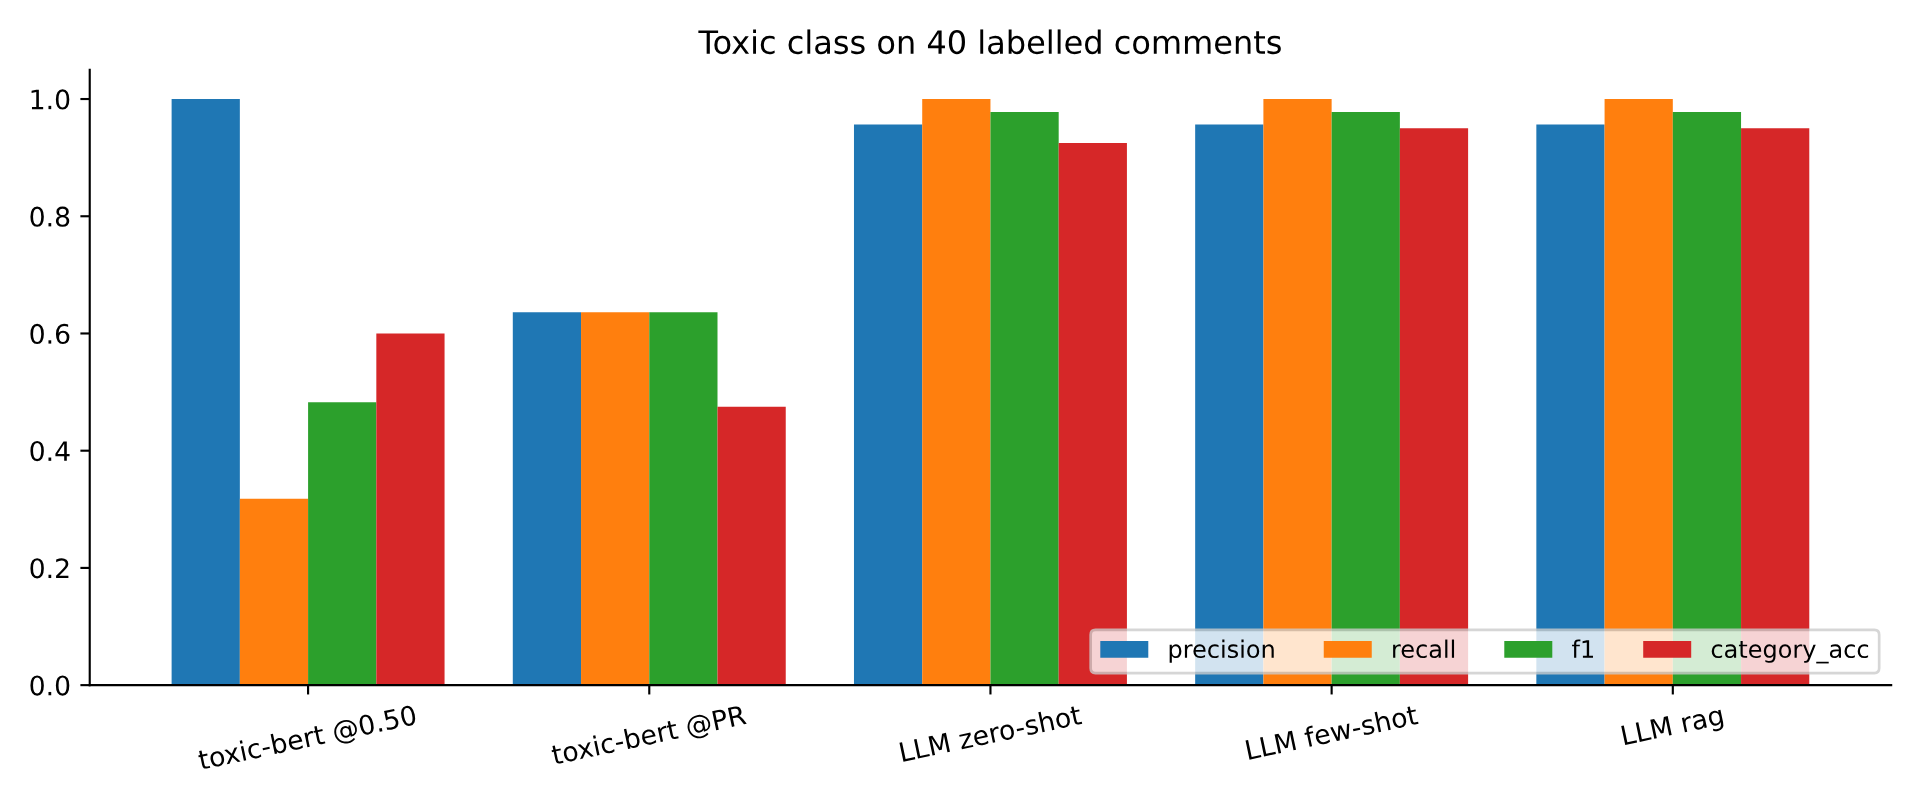
\includegraphics[width=\linewidth]{classification.png}
  \caption{Precision, recall, F1 i zgodność kategorii dla wszystkich wariantów.}
\end{figure}

\begin{table}[H]
\centering
\small
\begin{tabular}{@{}lccc@{}}
\toprule
Wariant & EN (9 naruszeń) & PL (13 naruszeń) & \\
\midrule
toxic-bert, próg 0,50 & 0,714 & 0,267 & \\
LLM few-shot & 1,000 & 0,963 & \\
\bottomrule
\end{tabular}
\caption{F1 osobno dla komentarzy angielskich i polskich.}
\end{table}

\begin{table}[H]
\centering
\small
\begin{tabular}{@{}lccc@{}}
\toprule
Wyszukiwarka & Recall@1 & Recall@3 & MRR \\
\midrule
BM25 & 0,350 & 0,650 & 0,546 \\
embeddingi (\kod{nomic-embed-text}) & 0,525 & \textbf{0,850} & 0,682 \\
hybryda RRF & 0,500 & 0,775 & 0,670 \\
\bottomrule
\end{tabular}
\caption{Czy właściwy paragraf jest wśród znalezionych.}
\end{table}

\subsection{Co z tego wynika}

\begin{itemize}
  \item \textbf{toxic-bert} przy progu 0,5 nie myli się, gdy coś oznaczy (precision 1,0), ale łapie tylko co trzecie
        naruszenie. Dla polskich komentarzy F1 to 0,27 -- model zna tylko angielski. Nie rozpoznaje też spamu, bo
        nie ma takiej etykiety. Próg dobrany z krzywej PR wyrównuje precision i recall, ale przy 0,056 oznacza już
        dużo poprawnych komentarzy.
  \item \textbf{LLM} jest dużo lepszy we wszystkich wariantach. Jedynym fałszywym alarmem jest
        ,,Kurde, znowu zapomniałem średnika. Klasyka.'' -- model uznał lekkie przekleństwo za naruszenie (decyzja
        \kod{review}, nie \kod{remove}). Na 40 komentarzach zero-shot, few-shot i RAG mają po poprawkach tę samą
        F1, więc ten zbiór jest za mały, żeby je rozróżnić w samym wykrywaniu.
  \item \textbf{RAG} nie poprawia wykrywania, ale dodaje to, czego brakuje pozostałym wariantom: podstawę decyzji.
        Właściwy paragraf wskazał w 85\% komentarzy. Kosztuje to dwa razy więcej czasu (embedding zapytania i dłuższy
        prompt).
  \item \textbf{Wyszukiwanie}: embeddingi wygrały z BM25, a hybryda wypadła gorzej niż same embeddingi. BM25 słabo
        radzi sobie z angielskim spamem w porównaniu z polskim regulaminem (1 trafienie na 5), a RRF przenosi ten
        błąd do wyniku łącznego. Dlatego domyślną metodą w \kod{config.yaml} jest \kod{dense}.
\end{itemize}

Uczciwie trzeba dodać, że prompt, wybór wyszukiwarki i stałe dołączanie §2.3 ustalałem, patrząc na ten sam zbiór
40 komentarzy, więc wyniki RAG są raczej optymistyczne. Jeden komentarz to 2,5 punktu procentowego.

\newpage
\section{Aplikacja webowa}
\label{sec:aplikacja}

Polecenie \kod{moderator web} (w Dockerze uruchamiane automatycznie) startuje aplikację Gradio pod adresem
\url{http://localhost:7860}. Nagłówek pokazuje używane modele i to, czy Ollama odpowiada, więc brakujący model widać
od razu. Każda zakładka jest osobnym plikiem w \kod{src/moderator/web/tabs/} i korzysta z tej samej klasy
\kod{Moderator} co terminal. Wynik oceny ma postać karty: kolor i plakietka decyzji, pasek stopnia naruszenia,
uzasadnienie, kategorie i -- w trybie RAG -- cytowany paragraf razem z jego treścią. Przyciski nad nagłówkiem
przełączają język interfejsu (PL / EN) oraz motyw jasny i ciemny; wybór zapamiętuje przeglądarka. Zmienia się tylko
interfejs, a komentarze, odpowiedzi modelu i regulamin zostają bez zmian.

\zrzut{web_01_single_comment}{Zakładka \emph{Single comment}: groźba oceniona w trybie RAG z cytowanym paragrafem.}

\zrzut{web_02_image}{Zakładka \emph{Image}: tekst odczytany ze zrzutu ekranu i jego ocena.}

\zrzut{web_03_batch}{Zakładka \emph{Batch}: statystyki, wykres, tabela i pliki wynikowe dla 40 komentarzy.}

\zrzut{web_04_chat}{Zakładka \emph{Chat about a file}: pytanie o groźby, dopytanie z historią i zapisane pliki.}

\zrzut{web_05_rules}{Zakładka \emph{Rules (RAG)}: wyszukiwanie paragrafów i cały regulamin.}

\zrzut{web_06_evaluation}{Zakładka \emph{Evaluation}: wyniki \kod{moderator evaluate}.}

\section{Wnioski i ograniczenia}

\begin{enumerate}
  \item Lokalny model 7B w Ollamie wystarcza do moderacji po polsku i po angielsku. Na 40 komentarzach wykrył
        wszystkie naruszenia (recall 1,0) z jednym fałszywym alarmem, podczas gdy \kod{unitary/toxic-bert} z
        laboratorium 2 wykrył co trzecie, a po polsku prawie nic.
  \item Największy wpływ na jakość miały dwie małe zmiany w prompcie i schemacie, a nie wybór trybu: definicja pola
        \kod{toxic} (F1 zero-shot z 0,878 do 0,978) oraz ograniczenie pola \kod{rule} do znalezionych paragrafów
        (zgodność paragrafu z 0,60 do 0,85).
  \item Wymuszony schemat JSON (\kod{format}) jest ważniejszy niż temperatura: bez niego żadna z 5 odpowiedzi nie
        miała pełnego formatu, a z nim decyzja nie zmieniała się nawet przy $T = 1{,}5$.
  \item RAG nie zwiększył liczby wykrytych naruszeń, ale dał to, czego moderator potrzebuje do decyzji: wskazanie
        paragrafu. Błędy zostały w miejscach, gdzie paragrafy są do siebie podobne (§5.1 i §5.2, §4.1 i §4.2, §3.1
        i §3.2). Raz model usunął komentarz, cytując paragraf o dozwolonej krytyce (§2.3) -- taką niespójność warto
        by w przyszłości też wykrywać w kodzie.
  \item W wyszukiwaniu najlepiej wypadły same embeddingi; BM25 przegrywa, gdy komentarz jest po angielsku,
        a regulamin po polsku, i ciągnie w dół ranking hybrydowy.
  \item W rozmowie o pliku model dobrze znajduje i tłumaczy konkretne komentarze, ale myli się przy liczeniu.
        Liczby w raportach liczy więc kod.
\end{enumerate}

Ograniczenia:
\begin{itemize}
  \item zbiór testowy jest mały (40 komentarzy) i syntetyczny, a prompt i wyszukiwarkę dobierałem na tym samym
        zbiorze, więc liczby są raczej optymistyczne,
  \item \kod{nomic-embed-text} jest modelem głównie angielskim; dla polskiego regulaminu lepszy byłby model
        wielojęzyczny (np. \kod{bge-m3}),
  \item na procesorze (Docker na macOS, komputer bez GPU) ocena jednego komentarza trwa kilkadziesiąt sekund zamiast
        kilku,
  \item uzasadnienia po polsku czasem zawierają błędy językowe; większy model albo polski Bielik prawdopodobnie by to
        poprawił.
\end{itemize}

Możliwe rozszerzenia: większy, ręcznie oznaczony zbiór testowy, wielojęzyczne embeddingi, sprawdzanie uzasadnienia
modelem NLI zdanie po zdaniu (wniosek z laboratorium 5.3) i kontrola zgodności decyzji z cytowanym paragrafem.

\end{document}
